% SemEval-2027 Task 1 (RETECO) system description paper — ACL format.
% Compile: latexmk -pdf main.tex   (or upload the paper/ folder to Overleaf)
\documentclass[11pt]{article}

% "review" = anonymous submission; "final" = camera-ready; "preprint" = arXiv / course report.
\usepackage[final]{acl}

\usepackage{times}
\usepackage{latexsym}
\usepackage[T1]{fontenc}
\usepackage[utf8]{inputenc}
\usepackage{microtype}
\usepackage{inconsolata}
\usepackage{graphicx}
\usepackage{booktabs}
\usepackage{multirow}
\usepackage{amsmath,amssymb}
\usepackage{xcolor}
\usepackage{xspace}
\usepackage{tikz}
\usetikzlibrary{positioning,arrows.meta}

\newcommand{\sys}{\textsc{ChronoFuse}\xspace}
\newcommand{\todo}[1]{\textcolor{red}{[TODO: #1]}}
% generated by scripts/make_tables.py
\newcommand{\finalRerankA}{Qwen3-Reranker-4B}
\newcommand{\finalRerankB}{BGE-reranker-v2-m3}
\newcommand{\gainBmA}{89}
\newcommand{\gainBmB}{53}
\newcommand{\gainOfficialA}{224}
\newcommand{\gainOfficialB}{190}
\newcommand{\pFinalDenseA}{$<$\,0.001}
\newcommand{\pFinalDenseB}{$<$\,0.001}
\newcommand{\pctGoldOverlap}{34\%}
\newcommand{\pctTopOverlap}{43\%}
\newcommand{\pctdocyear}{40\%}
\newcommand{\plannerEvents}{2.2}
\newcommand{\plannerIntentAcc}{34\%}
\newcommand{\plannerWindowHit}{76\%}
\newcommand{\poolChannelsA}{dense, LLM-PRF query2doc ($\times$0.5), dense document vectors ($\times$0.5), LLM multi-query ($\times$0.5)}
\newcommand{\poolChannelsB}{dense, LLM-PRF query2doc, temporal RAPTOR ($\times$0.5), LLM query2doc ($\times$0.5)}
\newcommand{\rBgeA}{.215}
\newcommand{\rBgeB}{.275}
\newcommand{\rBgePoolA}{.277}
\newcommand{\rBgePoolB}{.317}
\newcommand{\rBmA}{.197}
\newcommand{\rBmB}{.223}
\newcommand{\rBmDenseA}{.281}
\newcommand{\rBmDenseB}{.309}
\newcommand{\rBmKgA}{.161}
\newcommand{\rBmKgB}{.190}
\newcommand{\rBmTimeA}{.168}
\newcommand{\rBmTimeB}{.205}
\newcommand{\rBmYhalfA}{.195}
\newcommand{\rBmYhalfB}{.221}
\newcommand{\rBmYzeroA}{.192}
\newcommand{\rBmYzeroB}{.216}
\newcommand{\rDenseA}{.297}
\newcommand{\rDenseB}{.314}
\newcommand{\rDenseDocA}{.306}
\newcommand{\rDenseDocB}{.312}
\newcommand{\rFinalA}{.371}
\newcommand{\rFinalB}{.341}
\newcommand{\rKgA}{.069}
\newcommand{\rKgB}{.070}
\newcommand{\rKwA}{.231}
\newcommand{\rKwB}{.218}
\newcommand{\rKwFbA}{.229}
\newcommand{\rKwFbB}{.222}
\newcommand{\rLateBgeA}{.289}
\newcommand{\rLateBgeB}{.341}
\newcommand{\rLateMiniLMA}{.280}
\newcommand{\rLateMiniLMB}{.315}
\newcommand{\rLateQbigA}{.371}
\newcommand{\rLateQbigB}{--}
\newcommand{\rLateQsmallA}{.347}
\newcommand{\rLateQsmallB}{.352}
\newcommand{\rListwiseA}{--}
\newcommand{\rListwiseB}{--}
\newcommand{\rMiniLMA}{.179}
\newcommand{\rMiniLMB}{.233}
\newcommand{\rMiniLMPoolA}{.258}
\newcommand{\rMiniLMPoolB}{.296}
\newcommand{\rMultiA}{.218}
\newcommand{\rMultiB}{.224}
\newcommand{\rMultiFbA}{.244}
\newcommand{\rMultiFbB}{.237}
\newcommand{\rOfficialA}{.115}
\newcommand{\rOfficialB}{.118}
\newcommand{\rPoolA}{.332}
\newcommand{\rPoolB}{.325}
\newcommand{\rPriorExpA}{.197}
\newcommand{\rPriorExpB}{.223}
\newcommand{\rPriorTprfA}{.197}
\newcommand{\rPriorTprfB}{.223}
\newcommand{\rQbigRRA}{.352}
\newcommand{\rQbigRRB}{--}
\newcommand{\rQbigRRPoolA}{.352}
\newcommand{\rQbigRRPoolB}{--}
\newcommand{\rQsmallRRA}{.283}
\newcommand{\rQsmallRRB}{.319}
\newcommand{\rQsmallRRPoolA}{.320}
\newcommand{\rQsmallRRPoolB}{.341}
\newcommand{\rQtdA}{.239}
\newcommand{\rQtdB}{.216}
\newcommand{\rQtdFbA}{.242}
\newcommand{\rQtdFbB}{.223}
\newcommand{\rRaptorA}{.287}
\newcommand{\rRaptorB}{.301}
\newcommand{\rRaptorTA}{.290}
\newcommand{\rRaptorTB}{.299}
\newcommand{\rRecallBmA}{.520}
\newcommand{\rRecallBmB}{.614}
\newcommand{\rRecallFinalA}{.743}
\newcommand{\rRecallFinalB}{.817}
\newcommand{\rRecallPoolA}{.738}
\newcommand{\rRecallPoolB}{.825}
\newcommand{\rRmA}{.177}
\newcommand{\rRmB}{.209}
\newcommand{\rTrainFinalA}{.302}
\newcommand{\rTrainFinalB}{.310}

\title{\sys at SemEval-2027 Task 1: Passages, Neighbouring Events and LLM Reranking
       Beat Date Matching for Temporal Reasoning-Intensive Retrieval}

\author{Ahmet \"{O}nder \"{O}nl\"{u} \\
  Istanbul Technical University \\
  \texttt{onlu26@itu.edu.tr}}

\begin{document}
\maketitle

\begin{abstract}
Temporal reasoning-intensive retrieval asks for evidence that is not only on topic but useful
for the period and events a question depends on. We describe \sys, our system for both
sub-tracks of RETECO Track~1 (SemEval-2027 Task~1), and use it to test, on all 13 domains and
1.17M documents, which retrieval ideas transfer to this setting: date-based structures (a year
index, a temporal knowledge graph, temporal priors and temporal pseudo-relevance feedback),
a time-aware RAPTOR tree, LLM query planning with event chains, multi-query, query2doc and
LLM-based feedback, dense retrieval, and encoder vs.\ decoder rerankers that select the top-10
from a top-100. Matching dates does not help: gold documents overlap the query's years
\emph{less} often than the non-relevant documents BM25 ranks highly. What helps is retrieval
granularity (passage-level BM25 lifts the official baseline from \rOfficialA{} to \rBmA{}
nDCG@10), semantic retrieval (\rDenseA{}) and \AbstractRerank{} With every choice made on train,
\sys reaches \rFinalA{} (1a) and \rFinalB{} (1b) nDCG@10 on dev, \gainOfficialA\% and
\gainOfficialB\% above the official baseline.
\end{abstract}

\section{Introduction}
\label{sec:intro}

For temporally grounded questions---``Why did the number of transactions per block jump in
2023?''---a passage on the right topic but about the wrong period is misleading evidence.
Track~1 of RETECO (SemEval-2027 Task~1; \citealp{reteco2027task}) operationalises this with
TEMPO \citep{abdallah2026tempo}, a 13-domain benchmark of English StackExchange questions whose
relevant documents must be both topical and temporally useful. The official BM25 baseline
reaches only \rOfficialA{} (Sub-track~1a) and \rOfficialB{} (1b) nDCG@10 on dev.

A natural reading of the task is that systems should \emph{match time}. We tested this with
rule-based years and with periods a small LLM infers for every document and question, and found
that it does not help: among questions that mention a year, only \pctGoldOverlap{} of gold
documents mention a year within $\pm1$ of it, against \pctTopOverlap{} of the non-relevant
documents in BM25's top~10 (Table~\ref{tab:data}). Relevant evidence describes the events
behind a question, often without repeating its dates.

\sys is built on that observation. It retrieves 200-word passages, which alone lifts BM25 from
\rOfficialA{} to \rBmA{} (1a); adds a dense embedder and a reasoning-trained retriever
(ReasonIR-8B); lets an LLM expand each question with a hypothetical answer, sub-queries and the
events \emph{neighbouring} it; fuses the channels selected on train; and reranks the top-100
with a decoder LLM. It reaches \rFinalA{} (1a) and \rFinalB{} (1b) nDCG@10 on dev, and
\pooledFinalA{} on all 1{,}730 TEMPO questions, above all twelve retrievers on the TEMPO
leaderboard (Table~\ref{tab:tempo}). Our contributions are (i)~a system evaluated on all 13
domains without sub-sampling, (ii)~evidence that date matching is not a useful relevance signal
on TEMPO, and (iii)~a comparison of encoder cross-encoders and decoder LLM rerankers on the same
candidates. Code is open.\footnote{\url{https://github.com/ITU-NLP-Team/nlp-term-project}}

\section{Background}
\label{sec:background}

\begin{figure*}[t]
  \centering
  \resizebox{\textwidth}{!}{%
  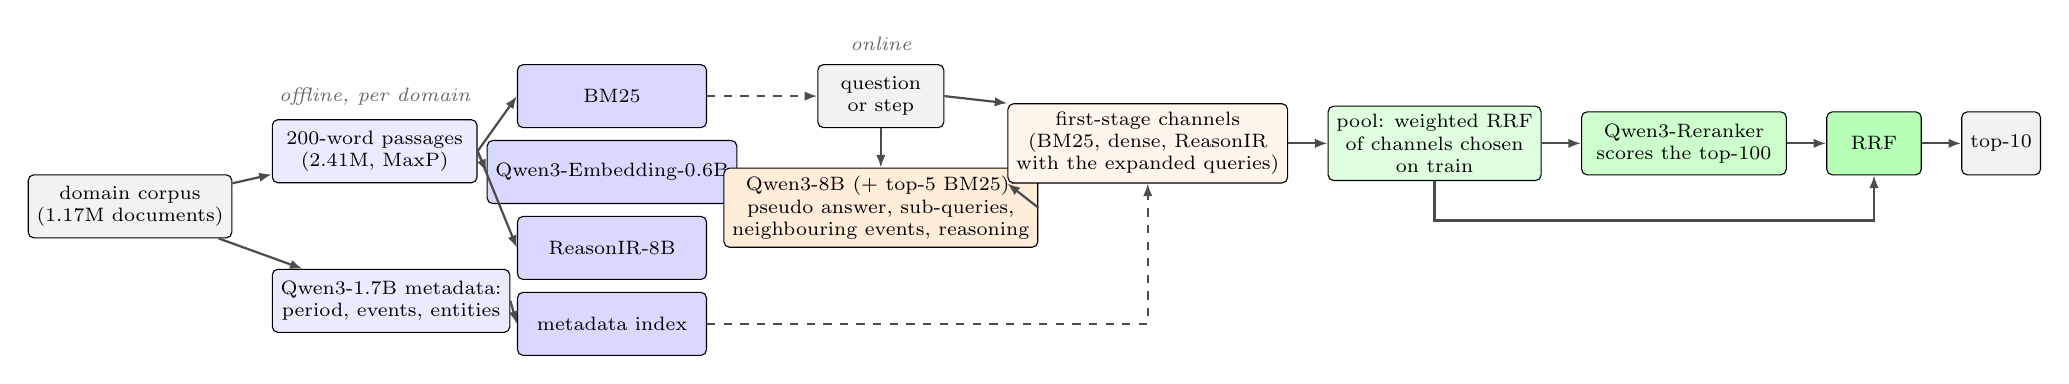
\begin{tikzpicture}[
      node distance=3mm and 5mm,
      box/.style={draw, rounded corners=2pt, align=center, font=\scriptsize,
                  minimum height=8mm, inner sep=3pt, fill=#1},
      box/.default=white,
      lab/.style={font=\scriptsize\itshape, text=black!60},
      arr/.style={-{Latex[length=1.6mm]}, thick, black!70}]
    % ---------------- offline
    \node[box=gray!10, minimum width=18mm] (corpus) {domain corpus\\(1.17M documents)};
    \node[box=blue!8, right=of corpus, yshift=7mm, minimum width=26mm] (chunk)
      {200-word passages\\(2.41M, MaxP)};
    \node[box=blue!8, right=of corpus, yshift=-12mm, minimum width=26mm] (meta)
      {Qwen3-1.7B metadata:\\period, events, entities};
    \node[box=blue!15, right=of chunk, yshift=7mm, minimum width=24mm] (bm25) {BM25};
    \node[box=blue!15, below=1.5mm of bm25, minimum width=24mm] (dense)
      {Qwen3-Embedding-0.6B};
    \node[box=blue!15, below=1.5mm of dense, minimum width=24mm] (rir) {ReasonIR-8B};
    \node[box=blue!15, below=1.5mm of rir, minimum width=24mm] (mindex) {metadata index};
    \draw[arr] (corpus) -- (chunk); \draw[arr] (corpus) -- (meta);
    \draw[arr] (chunk.east) -- (bm25.west); \draw[arr] (chunk.east) -- (dense.west);
    \draw[arr] (chunk.east) -- (rir.west); \draw[arr] (meta.east) -- (mindex.west);
    \node[lab, above=0.5mm of chunk] {offline, per domain};
    % ---------------- online
    \node[box=gray!10, right=14mm of bm25, minimum width=16mm] (q) {question\\or step};
    \node[box=orange!15, below=5mm of q, minimum width=30mm] (llm)
      {Qwen3-8B (+ top-5 BM25):\\pseudo answer, sub-queries,\\neighbouring events,
       reasoning};
    \node[lab, above=0.5mm of q] {online};
    \node[box=orange!8, right=8mm of q, yshift=-6mm, minimum width=30mm] (chan)
      {first-stage channels\\(BM25, dense, ReasonIR\\with the expanded queries)};
    \node[box=green!12, right=of chan, minimum width=22mm] (pool)
      {pool: weighted RRF\\of channels chosen\\on train};
    \node[box=green!20, right=of pool, minimum width=26mm] (rr)
      {Qwen3-Reranker\\scores the top-100};
    \node[box=green!28, right=of rr, minimum width=12mm] (fin) {RRF};
    \node[box=gray!10, right=of fin, minimum width=10mm] (out) {top-10};
    \draw[arr] (q) -- (llm);
    \draw[arr] (q.east) -- (chan.north west);
    \draw[arr] (llm.east) -- (chan.south west);
    \draw[arr] (chan) -- (pool); \draw[arr] (pool) -- (rr); \draw[arr] (rr) -- (fin);
    \draw[arr] (pool.south) -- ++(0,-5mm) -| (fin.south);
    \draw[arr] (fin) -- (out);
    \draw[arr, dashed] (bm25.east) -- (q.west);
    \draw[arr, dashed] (mindex.east) -| (chan.south);
  \end{tikzpicture}}
  \caption{\sys. Offline: passages, BM25, two dense indexes and an LLM metadata index. Online:
  Qwen3-8B expands the question; the train-selected channels are fused into a pool whose top-100
  a decoder reranker rescores.}
  \label{fig:overview}
\end{figure*}

\paragraph{Task.} Each of TEMPO's 13 domains has its own corpus (1{,}167{,}159 documents in
RETECO v1.1). Sub-track~1a ranks documents for the whole question, Sub-track~1b for each step of
an annotated reasoning decomposition. Relevance is binary; the metric is nDCG@10, averaged per
domain and macro-averaged over domains. Train/dev splits are 70/30 per domain and the test set is
hidden. Train/dev queries come with \emph{query guidance} (temporal intent, anchors, events, a
retrieval plan) that is not available at test time.

\paragraph{Related work.} BM25 \citep{robertson2009bm25} with passage-level MaxP scoring
\citep{dai2019maxp}, dense \citep{karpukhin2020dpr,zhang2025qwen3emb} and reasoning-trained
retrievers \citep{su2025bright,shao2025reasonir} are combined with reciprocal rank fusion
(RRF; \citealp{cormack2009rrf}). LLMs expand queries with hypothetical documents
\citep{gao2023hyde,wang2023query2doc} or sub-queries \citep{rackauckas2024ragfusion}, and rerank
as cross-encoders \citep{nogueira2019passage} or decoders \citep{nogueira2020monot5,zhang2025qwen3emb}.
Time-aware ranking combines text relevance with a temporal similarity between query and document
\citep{campos2014survey,jones2007temporal}. TEMPO reports that a reasoning retriever gains most
when the query is extended with an LLM's reasoning \citep{abdallah2026tempo}.

\section{System}
\label{sec:system}

\begin{figure*}[t]
  \centering
  \resizebox{\textwidth}{!}{%
  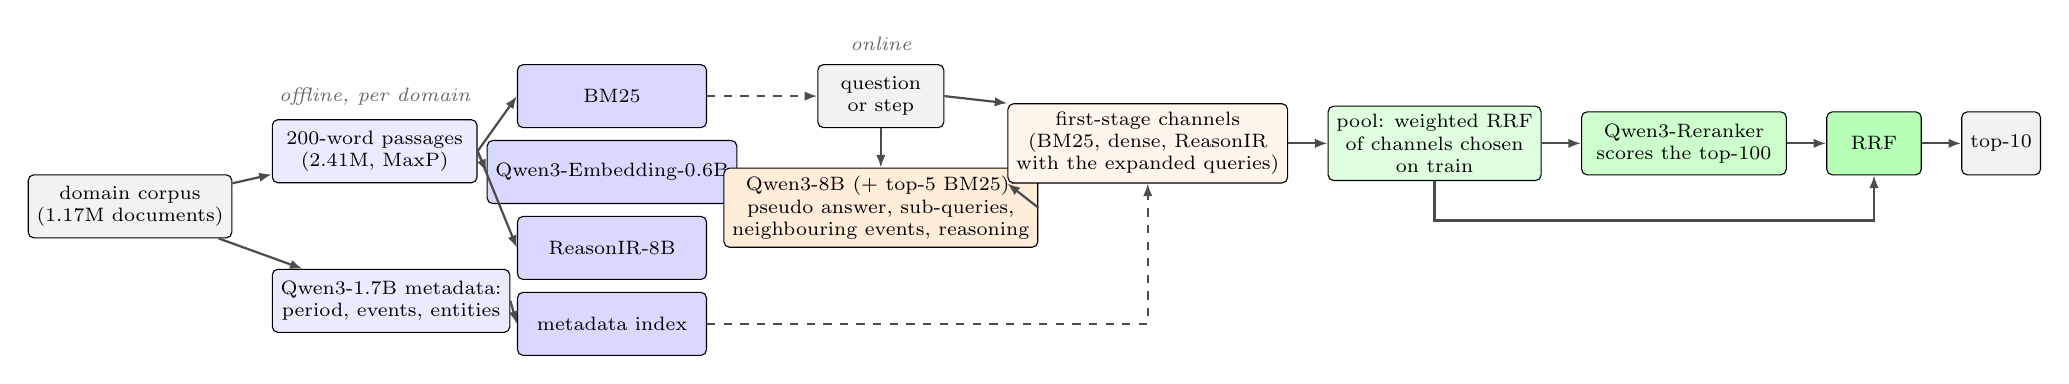
\begin{tikzpicture}[
      node distance=3mm and 5mm,
      box/.style={draw, rounded corners=2pt, align=center, font=\scriptsize,
                  minimum height=8mm, inner sep=3pt, fill=#1},
      box/.default=white,
      lab/.style={font=\scriptsize\itshape, text=black!60},
      arr/.style={-{Latex[length=1.6mm]}, thick, black!70}]
    % ---------------- offline
    \node[box=gray!10, minimum width=18mm] (corpus) {domain corpus\\(1.17M documents)};
    \node[box=blue!8, right=of corpus, yshift=7mm, minimum width=26mm] (chunk)
      {200-word passages\\(2.41M, MaxP)};
    \node[box=blue!8, right=of corpus, yshift=-12mm, minimum width=26mm] (meta)
      {Qwen3-1.7B metadata:\\period, events, entities};
    \node[box=blue!15, right=of chunk, yshift=7mm, minimum width=24mm] (bm25) {BM25};
    \node[box=blue!15, below=1.5mm of bm25, minimum width=24mm] (dense)
      {Qwen3-Embedding-0.6B};
    \node[box=blue!15, below=1.5mm of dense, minimum width=24mm] (rir) {ReasonIR-8B};
    \node[box=blue!15, below=1.5mm of rir, minimum width=24mm] (mindex) {metadata index};
    \draw[arr] (corpus) -- (chunk); \draw[arr] (corpus) -- (meta);
    \draw[arr] (chunk.east) -- (bm25.west); \draw[arr] (chunk.east) -- (dense.west);
    \draw[arr] (chunk.east) -- (rir.west); \draw[arr] (meta.east) -- (mindex.west);
    \node[lab, above=0.5mm of chunk] {offline, per domain};
    % ---------------- online
    \node[box=gray!10, right=14mm of bm25, minimum width=16mm] (q) {question\\or step};
    \node[box=orange!15, below=5mm of q, minimum width=30mm] (llm)
      {Qwen3-8B (+ top-5 BM25):\\pseudo answer, sub-queries,\\neighbouring events,
       reasoning};
    \node[lab, above=0.5mm of q] {online};
    \node[box=orange!8, right=8mm of q, yshift=-6mm, minimum width=30mm] (chan)
      {first-stage channels\\(BM25, dense, ReasonIR\\with the expanded queries)};
    \node[box=green!12, right=of chan, minimum width=22mm] (pool)
      {pool: weighted RRF\\of channels chosen\\on train};
    \node[box=green!20, right=of pool, minimum width=26mm] (rr)
      {Qwen3-Reranker\\scores the top-100};
    \node[box=green!28, right=of rr, minimum width=12mm] (fin) {RRF};
    \node[box=gray!10, right=of fin, minimum width=10mm] (out) {top-10};
    \draw[arr] (q) -- (llm);
    \draw[arr] (q.east) -- (chan.north west);
    \draw[arr] (llm.east) -- (chan.south west);
    \draw[arr] (chan) -- (pool); \draw[arr] (pool) -- (rr); \draw[arr] (rr) -- (fin);
    \draw[arr] (pool.south) -- ++(0,-5mm) -| (fin.south);
    \draw[arr] (fin) -- (out);
    \draw[arr, dashed] (bm25.east) -- (q.west);
    \draw[arr, dashed] (mindex.east) -| (chan.south);
  \end{tikzpicture}}
  \caption{\sys. Offline, every document is split into passages, indexed with BM25 and two
  dense encoders, and summarised by a small LLM into a metadata record. Online, Qwen3-8B
  expands the question (given the top BM25 results); the expanded queries run through the
  indexes, a train-selected subset of these channels is fused into a pool, and a decoder
  reranker scores the pool's top-100, which is fused with the pool into the final top-10.}
  \label{fig:overview}
\end{figure*}

Figure~\ref{fig:overview} summarises \sys. It has three parts: indexes built once per domain
(\S\ref{sec:indexes}), first-stage channels that combine those indexes with LLM-expanded
queries (\S\ref{sec:channels}), and a train-selected pool reranked by a decoder LLM
(\S\ref{sec:pool}). Every component runs per domain and is cached, so all variants in
Table~\ref{tab:full} are evaluated on identical candidates.

\subsection{Indexes}
\label{sec:indexes}
\paragraph{Passages.} TEMPO documents range from a sentence to multi-megabyte dumps. We split
every document into 200-word passages with a 40-word overlap (at most 64 per document; 2.41M
passages in total) and score a document by its best passage (MaxP, \citealp{dai2019maxp}).
Passages after the first are prefixed with the document's title, so that they keep its topic.

\paragraph{BM25.} Lucene BM25 with the official parameters ($k_1{=}0.9$, $b{=}0.4$) over
passages, built with \texttt{bm25s} and a streaming index builder that reproduces its scores
exactly and fits the largest domain (\emph{history}, 200k documents) in memory.

\paragraph{Dense.} All passages are embedded with Qwen3-Embedding-0.6B
\citep{zhang2025qwen3emb} and, separately, with ReasonIR-8B \citep{shao2025reasonir}, a
Llama-3.1-8B encoder trained for reasoning-intensive retrieval. Search is exact (inner product
on GPU) followed by MaxP; for Qwen3-Embedding we also keep document vectors (the mean of a
document's passage vectors).

\paragraph{LLM metadata.} A small LLM (Qwen3-1.7B, \citealp{yang2025qwen3}) reads the opening of
every document (220 words, at most 1{,}600 characters) and returns, as JSON, the period the text
is \emph{about}---including implicit periods such as ``after the 2008 crisis''---up to five
events, six entities, six keywords and a subtopic. The events, entities, keywords and title of
each document form a short text that is indexed with BM25 at document level (the
\emph{metadata index}). The same prompt is applied to every question, so questions and
documents share one schema.

\subsection{Query Expansion and Channels}
\label{sec:channels}
All expansions come from Qwen3-8B \citep{yang2025qwen3} in non-thinking mode with greedy,
JSON-schema-guided decoding. Following LLM-based pseudo-relevance feedback, the prompts can
include the first 60 words of the top-5 BM25 documents, so that the model reuses the
vocabulary, names and dates the collection actually uses. Each expansion becomes a
\emph{channel}, a ranked list of 100 documents:

\begin{itemize}
  \setlength\itemsep{1pt}
  \item \textbf{query2doc}: BM25 with the question plus a 60--90-word hypothetical answer and
        8--15 keywords \citep{wang2023query2doc}, with or without BM25 feedback. A single
        demonstration, built from one train question of the same domain (its released
        guidance and its first gold document), shows the model the expected answer style.
  \item \textbf{Sub-queries}: the same prompt also returns three sub-queries and a
        chronological event chain; one BM25 run per sub-query and per event is fused with RRF, the
        question weighted twice \citep{rackauckas2024ragfusion}.
  \item \textbf{Neighbouring events}: relevant evidence often describes events \emph{around}
        the one a question names. A second prompt (with BM25 feedback) asks for 4--6 such
        events---causes, earlier, parallel and later events, each with a year---four
        period-anchored sub-queries and ten expansion terms. BM25 and Qwen3-Embedding runs for
        the question (weight 2), for every sub-query and for every event are fused with RRF.
  \item \textbf{ReasonIR}: the full question (for a step: question and step), and a second
        variant that appends Qwen3-8B's free-text reasoning about the question, as done with
        GPT-4o on TEMPO \citep{abdallah2026tempo}.
  \item \textbf{Dense} (Qwen3-Embedding, passages and document vectors) and the
        \textbf{metadata index}, queried with the question and its own small-LLM metadata.
\end{itemize}

\subsection{Pool and Reranking}
\label{sec:pool}
\paragraph{Pool.} Channels are combined with weighted reciprocal rank fusion
\citep{cormack2009rrf}, $s(d){=}\sum_c w_c/(60{+}\mathrm{rank}_c(d))$. Which channels enter, and
with which weight, is decided on the \emph{train} split by greedy forward selection: starting
from the best single channel, the (channel, $w\in\{1,\tfrac12\}$) pair that most improves train
macro nDCG@10 is added until no addition helps. Selection is run separately for 1a and 1b, over
all channels of Table~\ref{tab:full}.

\paragraph{Reranking.} The pool's top-100 is reranked pointwise and the reranked list is fused
with the pool by equal-weight RRF. Each candidate is shown as ``[first--last year] title $|$
best passage'', the best passage being the document's highest-scoring BM25 passage for the
question. We compare encoder \emph{cross-encoders}---MiniLM-L12 trained on MS~MARCO
\citep{wang2020minilm,nogueira2019passage} and BGE-reranker-v2-m3 \citep{chen2024bgem3}---with
decoder LLM rerankers, \emph{cross-decoders}: Qwen3-Reranker 0.6B and 4B \citep{zhang2025qwen3emb},
which read an instruction, the question and the document and score $P(\textit{yes})$ at the
answer position \citep[cf.][]{nogueira2020monot5}. Their instruction states RETECO's notion of
relevance (``evidence that helps answer it, including information about the relevant events and
time period''). The reranker is the one with the best train score for the sub-track;
reranking the BM25 $\oplus$ dense candidates instead of the pool's scored lower on train for the
selected rerankers.

\paragraph{Sub-track 1b.} A step is retrieved with ``title + step instruction'' (ReasonIR: full
question + step). The expansions, metadata and reasoning of the parent question are shared by
all of its steps.

\paragraph{Time-matching ablations.} To test whether explicit time helps, we also build
components that are \emph{not} part of the final system. A rule-based extractor normalises
years, ranges and dates in every document (in the final system it only supplies the year span
shown to the reranker); from it we build a year-filtered BM25, a year prior
$s'(d){=}(1{-}\lambda)\hat s(d){+}\lambda T(q,d)$ ($T$: fraction of the question's years the
document mentions, $\pm1$), and a document--entity--year graph searched with personalised
PageRank; with the LLM metadata, a period filter for BM25 and dense retrieval (overlap with the
question's period, $\pm2$ years, undated documents kept) and a period prior. $\lambda$ is chosen
on train. We also run RM3 pseudo-relevance feedback \citep{lavrenko2001relevance,abduljaleel2004umass}.

\section{Experimental Setup}
\label{sec:setup}

\paragraph{Data and protocol.} We use the latest RETECO release (v1.1, deduplicated Track~1
corpora) for all 13 domains, without sub-sampling: 1{,}211 train and 519 dev questions (1a) and
2{,}762 train and 1{,}214 dev steps (1b) over 1.17M documents (2.41M passages). Every choice
that is not fixed a priori---the pool's channels and weights, the reranker, RM3~$\alpha$ and the
prior weights of the ablations---is made on \textbf{train}, separately for 1a and 1b; dev is only
evaluated. Released guidance is used only to build the expansion prompt's demonstration (train) and for
post-hoc analysis (dev). Scoring follows the official protocol: \texttt{pytrec\_eval}
\texttt{ndcg\_cut\_10} \citep{vangysel2018pytreceval} per topic, topics missing from a run count
as zero, mean per domain, macro mean over domains; we also report recall@100. Significance is a
two-sided paired randomisation test over topics pooled across domains (10{,}000 permutations,
\citealp{smucker2007significance}). The official baseline is document-level Lucene BM25 with
the same $k_1$ and $b$ as ours.

\paragraph{Models.} All models are open-weight and none is fine-tuned on RETECO:
Qwen3-Embedding-0.6B (fp16, 384 tokens) and ReasonIR-8B (bf16, 512 tokens for passages, 1{,}024
for queries) as retrievers; Qwen3-8B and Qwen3-1.7B as generators (bf16, greedy,
non-thinking mode, served offline with vLLM~0.8.5); MiniLM-L12 (512 tokens), BGE-reranker-v2-m3,
Qwen3-Reranker-0.6B and -4B (1{,}024 tokens) as rerankers.

\paragraph{Compute.} All GPU work ran on the UHeM Altay cluster of Istanbul Technical University,
on nodes with four NVIDIA A100 80\,GB GPUs and 64 CPU cores, scheduled with SLURM;
Table~\ref{tab:compute} lists the cost of each stage. Indexes, vectors, models and caches take
93\,GB of storage in total. Within our allocation, the 4B reranker was run on train and dev 1a
and on 12 of the 13 dev domains of 1b, but not on the 2{,}762 train steps, so it is a candidate
for 1a only. The code also runs end to end on a CPU-only laptop (8\,GB RAM) with smaller
models, which we used for development.

\begin{table}[t]
\centering
\small
\setlength{\tabcolsep}{3pt}
\resizebox{\columnwidth}{!}{%
\begin{tabular}{llr}
\toprule
\textbf{Stage} & \textbf{Model} & \textbf{Cost} \\
\midrule
Embed 2.41M passages & Qwen3-Emb.-0.6B & 3.5 GPU-h \\
Embed 2.41M passages & ReasonIR-8B & 20 GPU-h \\
Metadata, 1.17M docs & Qwen3-1.7B & 11 GPU-h \\
Expansions, 1{,}730 questions & Qwen3-8B & 9 min / pass \\
Rerank 100 candidates & Qwen3-Rer.-0.6B & 1.05 s / topic \\
Rerank 100 candidates & Qwen3-Rer.-4B & 3.8 s / topic \\
\bottomrule
\end{tabular}}
\caption{Compute per stage on NVIDIA A100 80\,GB GPUs (GPU-h: A100-hours). BM25 indexing,
fusion and evaluation run on CPU.}
\label{tab:compute}
\end{table}

\section{Results}
\label{sec:results}

\begin{table}[t]
\centering
\small
\begin{tabular}{lr}
\toprule
Train queries & 1211 \\
\quad with an explicit year (rule extractor) & 43.4\% \\
\quad with a relative time expression & 65.6\% \\
\quad marked temporal in the guidance & 95.0\% \\
Gold documents per query & 3.60 \\
\midrule
Corpus documents with $\geq$1 year & 39.7\% \\
Gold documents with $\geq$1 year & 53.4\% \\
BM25 top-10 non-gold with $\geq$1 year & 65.4\% \\
\midrule
\multicolumn{2}{l}{\textit{Queries with an explicit year:}} \\
\quad gold docs overlapping a query year & 34.0\% \\
\quad BM25 top-10 non-gold overlapping & 42.6\% \\
\bottomrule
\end{tabular}
\caption{Temporal statistics of RETECO Track~1 (train). Gold evidence carries \emph{fewer} explicit years, and overlaps the query's years \emph{less} often, than the non-relevant documents BM25 ranks highly.}
\label{tab:data}
\end{table}
\begin{table}[t]
\centering
\small
\begin{tabular}{lcccc}
\toprule
 & \multicolumn{2}{c}{\textbf{1a}} & \multicolumn{2}{c}{\textbf{1b}} \\
\cmidrule(lr){2-3}\cmidrule(lr){4-5}
\textbf{System} & train & dev & train & dev \\
\midrule
BM25 (official) & .108 & .115 & .102 & .118 \\
BM25 passages + MaxP & .180 & .197 & .191 & .223 \\
Dense (Qwen3-Emb.-0.6B) & .231 & .297 & .246 & .314 \\
Hybrid pool (train-selected) & .273 & .332 & .305 & .325 \\
\sys (final) & .302 & .371 & .310 & .341 \\
\bottomrule
\end{tabular}
\caption{Macro nDCG@10 on RETECO Track~1 (v1.1).}
\label{tab:main}
\end{table}

Table~\ref{tab:main} gives the headline numbers; Table~\ref{tab:full} in
Appendix~\ref{app:full} lists every system with recall@100 and significance against our
passage-level BM25.

\paragraph{Passages explain most of the baseline gap.} Scoring 200-word passages with MaxP
instead of whole documents raises BM25 from \rOfficialA{} to \rBmA{} (1a) and from
\rOfficialB{} to \rBmB{} (1b) with the same $k_1$ and $b$. TEMPO documents include long dumps
whose length normalisation buries the one relevant paragraph; the gain is largest where the
official scores are near zero (\emph{bitcoin}, \emph{monero}, \emph{quant}, \emph{workplace};
Figure~\ref{fig:domains}).

\paragraph{Date matching does not help.} Every temporal device built on explicit years is
neutral or harmful when added to BM25: the prior's weight selected on train is (near) zero
(\rPriorExpA{} vs.\ \rBmA{}), temporal PRF does not change this (\rPriorTprfA{}), fusing the
year-index-filtered run costs \rBmA{}$\rightarrow$\rBmTimeA{}, and the temporal KG costs
\rBmA{}$\rightarrow$\rBmKgA{}. Down-weighting year tokens in the query is also slightly
harmful (\rBmYhalfA{}, \rBmYzeroA{}), so dates are useful query terms, but already exploited by
BM25. Table~\ref{tab:data} explains why: gold documents mention years \emph{less} often than
the non-relevant documents BM25 retrieves, and overlap the query's years less often
(\pctGoldOverlap{} vs.\ \pctTopOverlap{}). RM3 also hurts (\rRmA{}): feedback documents of
long StackExchange questions are noisy.

\paragraph{Dense retrieval is the strongest single channel.} Qwen3-Embedding-0.6B over
passages reaches \rDenseA{} (1a) and \rDenseB{} (1b), and its document-vector variant
\rDenseDocA{} (1a). Equal-weight fusion with BM25 is \emph{below} dense alone
(\rBmDenseA{}), which is why the pool is selected with weights on train.

\paragraph{Temporal RAPTOR.} The collapsed tree performs on par with flat dense retrieval
(\rRaptorA{}/\rRaptorTA{} for the plain/temporal tree on 1a, \rRaptorB{}/\rRaptorTB{} on 1b):
cluster smoothing and child expansion neither help nor hurt much when the leaves are already
strong, and adding the time dimension to the clustering changes little on its own. Its
value is complementarity: forward selection adds the temporal tree to the 1b pool, where its
cluster-expanded candidates raise recall beyond flat dense retrieval. Unlike LLM-summarised
RAPTOR, our centroid tree adds no new text to match against; we return to this in the
limitations.

\paragraph{LLM query planning.} Every LLM-derived channel beats BM25 on 1a:
query2doc reaches \rQtdA{}, keyword expansion \rKwA{} and multi-query with the event chain
\rMultiA{}, against \rBmA{}. Conditioning the planner on the top BM25 snippets (LLM-PRF) helps
consistently on train and gives the best 1a channels on dev (\rQtdFbA{} and \rMultiFbA{}),
while statistical feedback (RM3, \rRmA{}) hurts: the LLM keeps the vocabulary of the feedback
documents that fits the question and discards the rest. On 1b the gains shrink (\rMultiFbB{}
for LLM-PRF multi-query vs.\ \rBmB{}), since plans describe the parent question rather than
the step. The planner agrees with the gold temporal intent for \plannerIntentAcc{} of dev
queries and, when the gold anchors contain a year, its window covers one of them for
\plannerWindowHit{}; it produces \plannerEvents{} events per question on average. Alone, the
LLM channels stay below dense retrieval, but they are complementary to it: forward selection
adds LLM-PRF query2doc to the pool in both sub-tracks (next paragraph).

\paragraph{Hybrid pool.} Forward selection on train picks \poolChannelsA{} for 1a and
\poolChannelsB{} for 1b, reaching \rPoolA{} / \rPoolB{} on dev with recall@100 of
\rRecallPoolA{} / \rRecallPoolB{} (BM25: \rRecallBmA{} / \rRecallBmB{}).

\begin{table}[t]
\centering
\small
\setlength{\tabcolsep}{4pt}
\resizebox{\columnwidth}{!}{%
\begin{tabular}{llcccc}
\toprule
 & & \multicolumn{2}{c}{\textbf{1a dev}} & \multicolumn{2}{c}{\textbf{1b dev}} \\
\cmidrule(lr){3-4}\cmidrule(lr){5-6}
\textbf{Reranker} & & pure & $\oplus$pool & pure & $\oplus$pool \\
\midrule
none (BM25 $\oplus$ dense) & & \multicolumn{2}{c}{.281} & \multicolumn{2}{c}{.309} \\
MiniLM-L12 (33M) & enc. & .179$^{\dagger}$ & .258$^{\dagger}$ & .233$^{\dagger}$ & .296$^{\dagger}$ \\
BGE-v2-m3 (568M) & enc. & .215 & .277$^{\dagger}$ & .275$^{\dagger}$ & .317$^{\dagger}$ \\
Qwen3-Rerank. 0.6B & dec. & .283$^{\dagger}$ & .320$^{\dagger}$ & .319$^{\dagger}$ & .341$^{\dagger}$ \\
Qwen3-Rerank. 4B & dec. & .352$^{\dagger}$ & .352$^{\dagger}$ & -- & -- \\
\bottomrule
\end{tabular}}
\caption{Pointwise reranking of the same top-100 (BM25 $\oplus$ dense, RRF): encoder cross-encoders vs.\ decoder LLM rerankers (``cross-decoders''). \emph{pure}: sorted by the reranker; $\oplus$\emph{pool}: RRF of reranker and pool ranks. Macro nDCG@10, dev.}
\label{tab:rerank}
\end{table}

\paragraph{Cross-encoders vs.\ cross-decoders.} Table~\ref{tab:rerank} compares four rerankers
on the same top-100 (BM25 $\oplus$ dense, \rBmDenseA{} on 1a). The two encoder cross-encoders
\emph{hurt} when used alone (MiniLM \rMiniLMA{}, BGE-v2-m3 \rBgeA{}) and only approach the
candidate ranking when fused with it: trained on short web passages, they reward lexical
overlap with long StackExchange questions. The decoder rerankers, prompted with RETECO's
notion of relevance, improve on it: Qwen3-Reranker-0.6B reaches \rQsmallRRA{} alone and
\rQsmallRRPoolA{} fused, and the 4B model \rQbigRRA{} (\rQbigRRPoolA{} fused). On 1b the
picture is the same (\rMiniLMB{}, \rBgeB{} and \rQsmallRRB{} alone vs.\ \rBmDenseB{}). The gap
between the encoder and decoder families is larger than the gap between the two decoder sizes,
so the LLM backbone and the task instruction matter more than scale here.

\paragraph{Final system.} \sys fuses the train-selected pool with the candidates reranked by
the reranker whose fused system is best on train for the sub-track---\finalRerankA{} for 1a and
\finalRerankB{} for 1b (the 4B model is not a 1b candidate, see \S\ref{sec:setup}). It reaches
\rFinalA{} (1a) and \rFinalB{} (1b) nDCG@10 on dev with recall@100 of \rRecallFinalA{} /
\rRecallFinalB{}: \gainOfficialA\% / \gainOfficialB\% above the official baseline and
\gainBmA\% / \gainBmB\% above our passage BM25 (paired randomisation test against dense
retrieval: $p\,$\pFinalDenseA{} / $p\,$\pFinalDenseB{}). On train~1b the BGE and Qwen3-0.6B
fusions are tied (.310 vs.\ .309); on dev the latter would reach \rLateQsmallB{}, so the 1b
choice is conservative. All final-fusion variants are listed in Table~\ref{tab:full} (Appendix~\ref{app:full}).

\begin{figure}[t]
  \centering
  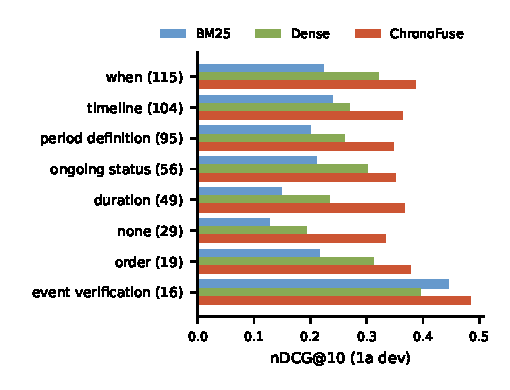
\includegraphics[width=\columnwidth]{figures/intent.pdf}
  \caption{nDCG@10 by gold temporal intent (1a dev; guidance used for analysis only).
  Number of queries in parentheses.}
  \label{fig:intent}
\end{figure}

\begin{figure*}[t]
  \centering
  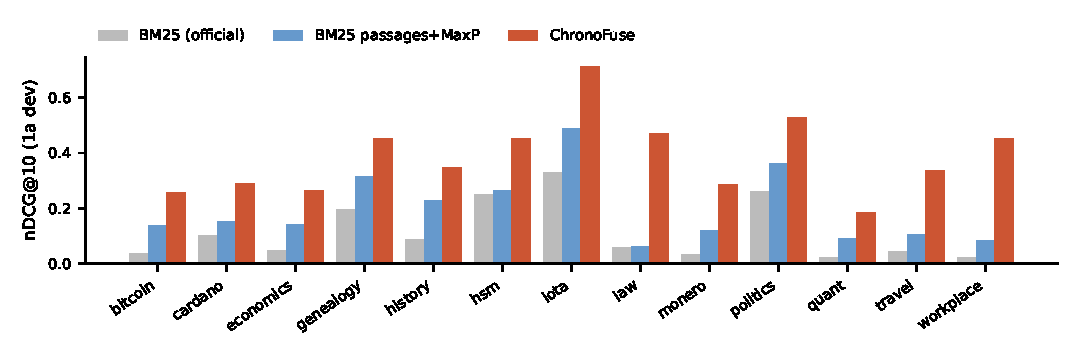
\includegraphics[width=0.9\textwidth]{figures/per_domain.pdf}
  \caption{Per-domain nDCG@10 on 1a dev: official document-level BM25, our passage BM25, and
  \sys.}
  \label{fig:domains}
\end{figure*}

\paragraph{Per-domain and per-intent analysis.} \sys improves over the official baseline and
over passage BM25 in every domain (Figure~\ref{fig:domains}); the largest absolute gains are on
\emph{law}, \emph{workplace} and \emph{iota} ($+$.23 to $+$.36 nDCG@10). By gold temporal intent (Figure~\ref{fig:intent}), the largest
gains over BM25 are for \emph{duration} (.149$\rightarrow$.361) and non-temporal questions
(.128$\rightarrow$.312), whose evidence rarely repeats the question's wording, followed by
\emph{when} and \emph{period definition}. The only intent where BM25 is competitive is
\emph{event verification} (16 questions), where the question names the event to be checked and
lexical matching already finds it.

\section{Conclusion}
\label{sec:conclusion}

We presented \sys, a retrieval and reranking system for RETECO Track~1 evaluated on the
complete data. Four findings stand out. (1)~Retrieval granularity matters more than temporal
machinery: passage-level BM25 alone improves the official baseline by more than 70\%.
(2)~Explicit dates are not a useful relevance signal on TEMPO---gold evidence mentions the
question's years less often than the documents BM25 already ranks highly---so year filters,
priors and graphs do not help, whether the dates come from rules or from an LLM. (3)~What
helps is semantics: a reasoning-trained retriever is the strongest single channel, and LLM
expansions---a hypothetical answer written with BM25 feedback and, above all, the events
neighbouring the question---add complementary candidates. (4)~To select the top-10 from a
top-100, decoder LLM rerankers prompted with the task's notion of relevance clearly beat encoder
cross-encoders, which \emph{hurt} on long StackExchange questions.

\sys reaches \rFinalA{} (1a) and \rFinalB{} (1b) nDCG@10 on dev, \gainOfficialA\% and
\gainOfficialB\% above the official baseline, and \pooledFinalA{} on all TEMPO questions, above
every retriever on the TEMPO leaderboard. The largest remaining gap is the quality of the
reasoning given to the reasoning-trained retriever; stronger reasoning, a reranker fine-tuned
on TEMPO's train judgments and the 4B reranker for steps are the next steps.

\section*{Limitations}
% Required by ACL; does not count toward the page limit.
\paragraph{Evaluation.} All numbers are on the released dev split; the hidden test set uses
newly annotated queries, so absolute scores may differ. Dev domains are small (3--240 queries),
so per-domain differences are noisy; we therefore report macro averages with a pooled
significance test and select every configuration on train.

\paragraph{Models and compute.} The generator (Qwen3-8B), the cross-decoders (0.6B/4B) and the
embedder (0.6B) are mid-sized open models; larger LLMs or reasoning-trained retrievers
\citep{shao2025reasonir} may change the ranking of components, in particular for query
planning and reranking. RAPTOR nodes are centroids rather than LLM summaries, which
was necessary at 1.17M documents but departs from the original method. GPU time on a shared
cluster also bounded the reranking study: the 4B cross-decoder is missing for 1b (train steps
and the \emph{history} dev steps), the final fusion reuses one reranking of the BM25 $\oplus$
dense candidates instead of re-scoring the selected pool, and a RankGPT-style listwise stage
with Qwen3-8B \citep{sun2023rankgpt}, implemented in our code, could not be evaluated at full
scale. LLM components add
latency and depend on a specific model version; all LLM outputs are cached for
reproducibility.

\paragraph{Temporal metadata.} Temporal profiles come from a rule-based extractor that misses
implicit periods expressed through events (``after the halving'') and may treat numbers such
as model years or block heights as dates. Entities are capitalised spans rather than linked
entities, which limits the knowledge graph.

\paragraph{Data.} All text is English StackExchange content; findings may not transfer to
other languages, genres or to temporally dense news corpora, where explicit dates are more
reliable signals.


\section*{Acknowledgments}
Computations were performed on the Altay cluster of the National Center for High Performance
Computing of Turkey (UHeM) at Istanbul Technical University.

\bibliography{references,reteco_refs}

\appendix
\section{Full Results}
\label{app:full}
\begin{table*}[t]
\centering
\small
\begin{tabular}{llcccc}
\toprule
 & & \multicolumn{2}{c}{\textbf{1a (whole query)}} & \multicolumn{2}{c}{\textbf{1b (step-wise)}} \\
\cmidrule(lr){3-4}\cmidrule(lr){5-6}
& \textbf{System} & nDCG@10 & R@100 & nDCG@10 & R@100 \\
\midrule
& BM25, document level (official baseline) & .115 & -- & .118 & -- \\
\midrule
\multicolumn{6}{l}{\textit{Lexical and pseudo-relevance feedback}} \\
& BM25 (passage, MaxP) & .197 & .520 & .223 & .614 \\
& BM25 + RM3 PRF ($\alpha{=}0.3$) & .177$^{\dagger}$ & .518 & .209$^{\dagger}$ & .630 \\
& BM25, 1b input = full query + step & -- & -- & .208$^{\dagger}$ & .644 \\
\midrule
\multicolumn{6}{l}{\textit{Temporal metadata (prior, year index, KG)}} \\
& BM25, year tokens $\times$0.5 & .195$^{\dagger}$ & .521 & .221$^{\dagger}$ & .612 \\
& BM25, year tokens removed & .192$^{\dagger}$ & .520 & .216$^{\dagger}$ & .606 \\
& BM25 + temporal prior (explicit years) ($\lambda{=}0.05$) & .197 & .520 & .223 & .614 \\
& BM25 + temporal prior (explicit or temporal PRF) ($\lambda{=}0.05$) & .197 & .520 & .223 & .614 \\
& year-index filtered BM25 (alone) & .039$^{\dagger}$ & .068 & .040$^{\dagger}$ & .080 \\
& BM25 $\oplus$ year-index filtered BM25 & .168$^{\dagger}$ & .512 & .205$^{\dagger}$ & .611 \\
& temporal KG (personalised PageRank) & .069$^{\dagger}$ & .153 & .070$^{\dagger}$ & .173 \\
& BM25 $\oplus$ temporal KG & .161$^{\dagger}$ & .484 & .190$^{\dagger}$ & .590 \\
\midrule
\multicolumn{6}{l}{\textit{Dense retrieval (Qwen3-Emb.-0.6B, ReasonIR-8B) and RAPTOR trees}} \\
& dense (Qwen3-Embedding-0.6B, passages) & .297$^{\dagger}$ & .710 & .314$^{\dagger}$ & .791 \\
& dense, document vectors & .306$^{\dagger}$ & .695 & .312$^{\dagger}$ & .766 \\
& RAPTOR tree (collapsed, no time) & .287$^{\dagger}$ & .698 & .301$^{\dagger}$ & .756 \\
& temporal RAPTOR tree & .290$^{\dagger}$ & .709 & .299$^{\dagger}$ & .764 \\
& BM25 $\oplus$ dense & .281$^{\dagger}$ & .697 & .309$^{\dagger}$ & .773 \\
& BM25 $\oplus$ temporal RAPTOR & .286$^{\dagger}$ & .706 & .305$^{\dagger}$ & .771 \\
& ReasonIR-8B (passages, full query) & .315$^{\dagger}$ & .762 & .326$^{\dagger}$ & .847 \\
& ReasonIR-8B + LLM reasoning query & .336$^{\dagger}$ & .745 & .321$^{\dagger}$ & .832 \\
& ReasonIR $\oplus$ ReasonIR + reasoning & .340$^{\dagger}$ & .767 & .330$^{\dagger}$ & .851 \\
\midrule
\multicolumn{6}{l}{\textit{LLM query planning (Qwen3-8B)}} \\
& LLM keyword expansion & .231$^{\dagger}$ & .588 & .218$^{\dagger}$ & .670 \\
& LLM query2doc & .239$^{\dagger}$ & .620 & .216$^{\dagger}$ & .656 \\
& LLM multi-query + event chain & .218 & .588 & .224 & .657 \\
& LLM-PRF keyword expansion & .229$^{\dagger}$ & .570 & .222$^{\dagger}$ & .671 \\
& LLM-PRF query2doc & .242$^{\dagger}$ & .593 & .223$^{\dagger}$ & .672 \\
& LLM-PRF multi-query + event chain & .244$^{\dagger}$ & .587 & .237 & .674 \\
\midrule
\multicolumn{6}{l}{\textit{Small-LLM metadata (Qwen3-1.7B) and neighbouring events (Qwen3-8B)}} \\
& BM25 + small-LLM events/entities/keywords & .226$^{\dagger}$ & .593 & .221 & .659 \\
& BM25 over LLM document metadata & .184$^{\dagger}$ & .587 & .196$^{\dagger}$ & .665 \\
& BM25, LLM-period filter & .195 & .499 & .217$^{\dagger}$ & .581 \\
& dense, LLM-period filter & .292$^{\dagger}$ & .664 & .303$^{\dagger}$ & .741 \\
& BM25 $\oplus$ dense + LLM-period prior ($\lambda{=}0.1$) & .287$^{\dagger}$ & .697 & .309$^{\dagger}$ & .773 \\
& BM25 $\oplus$ dense $\oplus$ metadata channels (filtered) & .279$^{\dagger}$ & .702 & .311$^{\dagger}$ & .793 \\
& neighbouring events + sub-queries (BM25) & .229$^{\dagger}$ & .630 & .229 & .732 \\
& neighbouring events + sub-queries (BM25 $\oplus$ dense) & .278$^{\dagger}$ & .750 & .269$^{\dagger}$ & .819 \\
\midrule
\multicolumn{6}{l}{\textit{Train-selected hybrid pool}} \\
& train-selected hybrid pool (RRF) & .346$^{\dagger}$ & .783 & .349$^{\dagger}$ & .873 \\
\midrule
\multicolumn{6}{l}{\textit{Pointwise reranking of the BM25 $\oplus$ dense top-100}} \\
& BM25 $\oplus$ dense $\rightarrow$ MiniLM-L12 cross-encoder & .179$^{\dagger}$ & .697 & .233$^{\dagger}$ & .773 \\
& BM25 $\oplus$ dense $\oplus$ MiniLM-L12 cross-encoder & .258$^{\dagger}$ & .697 & .296$^{\dagger}$ & .773 \\
& BM25 $\oplus$ dense $\rightarrow$ BGE-reranker-v2-m3 & .215 & .697 & .275$^{\dagger}$ & .773 \\
& BM25 $\oplus$ dense $\oplus$ BGE-reranker-v2-m3 & .277$^{\dagger}$ & .697 & .317$^{\dagger}$ & .773 \\
& BM25 $\oplus$ dense $\rightarrow$ Qwen3-Reranker-0.6B & .283$^{\dagger}$ & .697 & .319$^{\dagger}$ & .773 \\
& BM25 $\oplus$ dense $\oplus$ Qwen3-Reranker-0.6B & .320$^{\dagger}$ & .697 & .341$^{\dagger}$ & .773 \\
& BM25 $\oplus$ dense $\rightarrow$ Qwen3-Reranker-4B & .352$^{\dagger}$ & .697 & -- & -- \\
& BM25 $\oplus$ dense $\oplus$ Qwen3-Reranker-4B & .352$^{\dagger}$ & .697 & -- & -- \\
\midrule
\multicolumn{6}{l}{\textit{Final fusion: pool $\oplus$ reranked candidates}} \\
& selected pool $\oplus$ MiniLM-L12 cross-encoder & .294$^{\dagger}$ & .767 & .332$^{\dagger}$ & .866 \\
& selected pool $\oplus$ BGE-reranker-v2-m3 & .309$^{\dagger}$ & .763 & .355$^{\dagger}$ & .860 \\
& selected pool $\rightarrow$ BGE-reranker-v2-m3, $\oplus$ pool & .307$^{\dagger}$ & .783 & .357$^{\dagger}$ & .873 \\
& selected pool $\oplus$ Qwen3-Reranker-0.6B & .349$^{\dagger}$ & .767 & .367$^{\dagger}$ & .865 \\
& selected pool $\rightarrow$ Qwen3-Reranker-0.6B, $\oplus$ pool & .351$^{\dagger}$ & .783 & \textbf{.371$^{\dagger}$} & .873 \\
& selected pool $\oplus$ Qwen3-Reranker-4B & .382$^{\dagger}$ & .768 & -- & -- \\
& selected pool $\rightarrow$ Qwen3-Reranker-4B, $\oplus$ pool & \textbf{.387$^{\dagger}$} & .783 & -- & -- \\
& ChronoFuse (final, train-selected) & \textbf{.387$^{\dagger}$} & .783 & \textbf{.371$^{\dagger}$} & .873 \\
\bottomrule
\end{tabular}
\caption{Macro nDCG@10 and recall@100 on the RETECO Track~1 \textbf{dev} split (13 domains, v1.1). Hyper-parameters, the pool composition and the final configuration were selected on \textbf{train}. $^{\dagger}$: different from our passage BM25 at $p<0.05$ (paired randomisation test over queries/steps). $\oplus$: reciprocal rank fusion.}
\label{tab:full}
\end{table*}

\section{Prompts}
\label{app:prompts}

\paragraph{Query planner (system message).}
{\scriptsize\begin{verbatim}
You help a search engine answer time-sensitive questions
from a StackExchange forum. Read the question and return
ONLY a JSON object with these keys:
"temporal_intent": one of when, period_definition,
  timeline, ongoing_status, duration, before_after,
  order, none
"year_window": [first_year, last_year] the evidence
  should be about, or null
"events": chronological list of events the answer
  depends on, each {"year": int or null,
  "event": short phrase}
"keywords": 8-15 search keywords not already in the
  question (synonyms, names, versions, dates)
"sub_queries": 3 short search queries, each covering
  one part of the question
"answer_passage": a 60-90 word passage that would
  answer the question, with concrete names and dates
\end{verbatim}}
\noindent One demonstration follows: a train question of the same domain whose guidance
supplies the intent, events and sub-queries (TEMPO's retrieval plan), and whose first gold
document supplies the answer passage (first 80 words) and keywords (salient entities absent
from the question). Outputs are constrained to the JSON schema of these keys with vLLM guided
decoding (greedy, repetition penalty 1.05); truncated outputs are recovered field by field.
In the LLM-PRF variant the user turn ends with ``Top search results (may be noisy; reuse their
terms and dates):'' and the first 60 words of the top-5 BM25 documents.

\paragraph{Metadata extractor (Qwen3-1.7B, system message).}
{\scriptsize\begin{verbatim}
You extract search metadata from a text taken from a
StackExchange forum or the documents it cites. Return ONLY
a JSON object with these keys:
"start_year", "end_year": the period the text is ABOUT, as
  years. Infer implicit periods too (e.g. "after the 2008
  crisis" -> 2008-2010, "during the Weimar Republic" ->
  1919-1933). Use null for both if no period can be
  inferred.
"events": at most 5 short phrases naming the events,
  changes or releases the text discusses
"entities": at most 6 named people, organisations,
  products, laws, coins or places
"keywords": at most 6 topical search terms that are not
  entity names
"topic": a 2-5 word subtopic label
\end{verbatim}}

\paragraph{Neighbouring events (Qwen3-8B, system message).}
{\scriptsize\begin{verbatim}
You help a search engine find evidence for a time-sensitive
question. Relevant documents often describe related events
and mechanisms rather than repeating the question's words
or dates. Return ONLY a JSON object with these keys:
"period": [first_year, last_year] the evidence is about,
  or null
"neighbor_events": 4-6 events closely connected to the
  question (causes, preceding and following events,
  parallel developments), each {"event": short phrase with
  names, "year": int or null, "relation": one of cause,
  before, same_time, after, effect}
"sub_queries": 4 short self-contained search queries; each
  targets one event or aspect and names its period
"expansion_terms": 10 terms likely to appear in relevant
  documents that are not already in the question
\end{verbatim}}
\noindent The user turn contains the question and the first 60 words of the top-5 BM25
documents.

\paragraph{Reasoning for ReasonIR (Qwen3-8B, user message).}
{\scriptsize\begin{verbatim}
<question>
Instructions:
1. Identify the essential problem, including the time
   period and the events it depends on.
2. Think step by step to reason about what information
   relevant documents would contain (earlier and later
   events, causes, names, dates, mechanisms).
3. Draft an answer with as many thoughts as you have.
\end{verbatim}}

\paragraph{Cross-decoder instruction (Qwen3-Reranker).}
{\small ``Given a time-sensitive question from a StackExchange forum, judge whether the document
contains evidence that helps answer it, including information about the relevant events and
time period.''}

\section{Hyper-parameters}
\label{app:hparams}
\begin{table}[h]
\centering\small
\begin{tabular}{ll}
\toprule
Passages & 200 words, overlap 40, $\leq$64/doc \\
BM25 & Lucene, $k_1{=}0.9$, $b{=}0.4$, stem+stop \\
RM3 & 10 docs, 20 terms, $\alpha\in\{.3,.5,.7\}$ \\
Prior $\lambda$ & $\{0,.05,.1,.2,.3\}$, tolerance $\pm1$y \\
Temporal PRF & top-20, support $\geq$3, span $\leq$10y \\
Year-index filter & explicit query window, $\pm1$y \\
Temporal KG & entity df $\leq$5\%, PPR $\alpha{=}0.85$ \\
Dense & Qwen3-Emb.-0.6B, 384 tok, MaxP \\
ReasonIR & 8B, 512 tok (query 1{,}024), MaxP \\
LLM metadata & Qwen3-1.7B, 220 words / 1{,}600 chars \\
Period filter / prior & $\pm2$y; $\lambda\in\{0,.05,.1,.2,.3\}$ \\
RAPTOR & 2 levels, $\sim$10 children, $\beta{=}0.5$, \\
 & $\eta{=}0.3$, top-10 nodes expanded \\
RRF & $k{=}60$, weights $\in\{1,\tfrac12\}$ \\
Pointwise rerank & top-100 (BM25$\oplus$dense or pool), \\
 & best BM25 passage, 1{,}024 tokens \\
Final fusion & equal-weight RRF, late or pool \\
Generator & Qwen3-8B, greedy, non-thinking \\
\bottomrule
\end{tabular}
\caption{Hyper-parameters. Sets in braces are searched on train.}
\end{table}


\end{document}
